\section{Experiments}
\label{sec:experiments}
To fully verify the implementation of the proposed architecture, several experiments have been conducted. The experiments are strategically designed to test the effect of a set of features within a specific scenario. All experiments are executed in a simulated environment, from here on called a scenario. These scenarios allow us to reproduce the experiments in a controlled and predictable environment. The feature sets were chosen in such a way that they would individually help reason about their impact on the research questions from Subsection \ref{ssec:research-questions}. 

% Table \ref{table:experiments} shows a reference of the experiments that are executed, and how the scenarios and feature sets are combined.
% \begin{table}[H]
%     \begin{adjustwidth}{-1cm}{}
%         \centering
%         % \begin{table}[]
%         \begin{tabularx}{1.2\textwidth}{l|l|X|X|l}
%             \textbf{Feature sets \textbackslash Scenarios} & \textbf{No changes} & \textbf{Growing \newline Infrastructure} & \textbf{Unstable \newline Infrastructure} & \textbf{Mixed} \\ \hline
%             \textbf{Local}                             & A.1            & A.2                    & A.3                     & A.4   \\
%             \textbf{Knowledge-Sharing only}            & B.1            & B.2                    & B.3                     & B.4   \\
%             \textbf{Auctioning}                        & C.1            & C.2                    & C.3                     & C.4     
%         \end{tabularx}
        
%     \end{adjustwidth}
%     \caption{\label{table:experiments}Overview of the experiments that are conducted. Each scenario is conducted with a different set of features, to test the effect of the features on the results.}
% \end{table}

\subsection{Feature Sets}
Even though it would be interesting to test each feature individually, creating feature sets allowed us to focus on specific aspects of the implementation and reduce the number of experiments that needed to be conducted to a manageable number. 

The feature sets were chosen in a way that they relate to the research questions from Subsection \ref{ssec:research-questions}. The feature sets are defined as follows:

\begin{table}[H]
    % \begin{table}[]
        \centering
        \begin{tabular}{l|l|l|l}
            \textbf{Feature \textbackslash Set name} & \textbf{Local} & \textbf{Knowledge-Sharing} & \textbf{Auctioning} \\ \hline
            \textbf{Inspect host properties}     & yes            & yes                        & yes                 \\
            \textbf{Adapt host properties}       & yes            & yes                        & yes                 \\
            \textbf{Risk analysis}               & yes            & yes                        & yes                 \\
            \textbf{Share knowledge}             & no             & yes                        & yes                 \\
            \textbf{Initiate \& Join auctions}   & no             & no                         & yes                 \\
            \textbf{Migrate Software}            & no             & no                         & yes                            
        \end{tabular}
        \caption{\label{table:experiment-features}Overview of the actions that are allowed in each feature set. The headers of the table represent the names of the feature sets. The rows represent the actions that are allowed in each feature set.}
    % \end{table}
\end{table}

As shown in Table \ref{table:experiment-features}, the feature sets become increasingly complex. In the Local feature set, agents are only allowed to inspect and adapt their own properties and software components. In the Knowledge-Sharing feature set, agents are allowed to share knowledge with other agents. In the Auctioning feature set, agents are allowed to cooperate with other agents to mitigate risks through auctions.

From the table, it should also be visible that migrations of software can only be performed in the Auctioning feature set. This is because an agent on its own has insufficient knowledge and capabilities to perform a migration.

\subsection{Scenarios}
As mentioned before, each of the feature sets is executed in a specific scenario. A scenario is defined by an infrastructure and a set of events that will happen over time. These events could be new nodes joining the infrastructure, or nodes leaving the infrastructure. Because of the scenarios, it was possible to repeat the experiments over and over again without having to manually change the infrastructure. This allowed for better reasoning about- and comparing the results of each experiment. Additionally, it allowed for a more realistic approach to the experiments, as the infrastructure is not static and is changing over time.

Four scenarios have been defined, each with a different set of characteristics. These characteristics are defined as follows:

% \begin{description}
%     \item[No Changes]                 No infrastructure changes are made overtime.
%     \item[Growing Infrastructure]     The infrastructure is slowly growing over time.
%     \item[Unstable Infrastructure]    Some nodes in the infrastructure are unstable and are disconnected from the network from time to time.
%     \item[Mixed]                      A more realistic scenario where nodes are added and removed from the infrastructure over time.
% \end{description}

\paragraph*{No Changes}
This scenario is the simplest. In this scenario, the infrastructure is static and does not change over time. This means that no infrastructure nodes or software are added, and no links between them are removed. This scenario makes it possible to reason about the outcome of the experiments without having to take into account the changes in the infrastructure. 

\textit{This scenario runs for a maximum of 10 minutes, or until no messages have been sent for 1 minute. This means that the scenario will end when the agents have stopped communicating with each other. This is done to prevent the scenario from running indefinitely.}

\paragraph{Introduce Risks} 
In this scenario, risks are slowly introduced into the infrastructure to simulate the discovery of new CVEs. This is done by changing the properties of the existing nodes. No new infrastructure nodes or software are added. The properties that are changed to simulate new risks are properties that would trigger a risk rule to be identified. One example would be to set the \code{Contiki-NG OS} version of a property to a version that is known to have a vulnerability. This should trigger a risk rule that would identify a risk.
The update to the properties is done at exactly $120$ seconds after the start of the scenario. 

\textit{This scenario runs for a maximum of 10 minutes, no messages have been sent for 1 minute, or when the risk has been identified and mitigated.}

\paragraph*{Growing Infrastructure}
A more realistic scenario is one where the infrastructure is growing over time. This means that nodes are added to the infrastructure over time. The scenario has been hardcoded to add a new node to the infrastructure every 30 seconds\footnote{\label{footnote:simulation-time}These seconds are simulation time, see Section \ref{sssec:simulation-time} how this relates in real-time.} until a total of 5 nodes is added. When a node is added an existing node is picked semi-randomly, and an edge is made between the two.

\textit{After the last node has been added to the infrastructure, the scenario will finish when no messages have been sent for 1 minute, or when it has run for a maximum of 10 minutes. This is done to prevent the scenario from running indefinitely.}

\paragraph*{Unstable Infrastructure}
Another realistic scenario is one where the infrastructure is unstable. This means that nodes are removed from the infrastructure, but reappear after some time. The scenario has been hardcoded to remove a random node from the infrastructure every 30 seconds\footnote{See footnote [\ref{footnote:simulation-time}.} and add it back after 30 seconds. This is repeated two times in the scenario. This means that the infrastructure is flickering with the availability of nodes. This scenario is used to test the robustness of the system, and how it can deal with nodes that are not always available.

\textit{After the last node has been added to the infrastructure, the scenario will finish when no messages have been send for 1 minute, or when it has run for a maximum of 10 minutes. This is done to prevent the scenario from running indefinitely.}

% \paragraph*{Mixed}
% The last scenario is a combination of the previous scenarios. This means that nodes are added and removed from the infrastructure over time. 
% \add{Update the definition of the mixed scenario}

\subsection{Infrastructure}
\label{ssec:infrastructure}
The previous sections all mention that we rely on an infrastructure. This infrastructure is a carefully chosen set of nodes and links between them. Each with a set of properties that will help mimic a real-world infrastructure. The infrastructure is used in all of the experiments and is reset at the beginning of each experiment. It is important to note that the infrastructure is not static, and could change over time depending on the scenario.

The infrastructure that is used in the experiments is based on the infrastructure as used by Domb \cite{domb2019smart} with slight alterations to the properties of each infrastructure node, and can be seen in figure \ref{fig:infrastructure}. This exact infrastructure is used at the beginning of each experiment.

\begin{figure}[H]
    \centering
    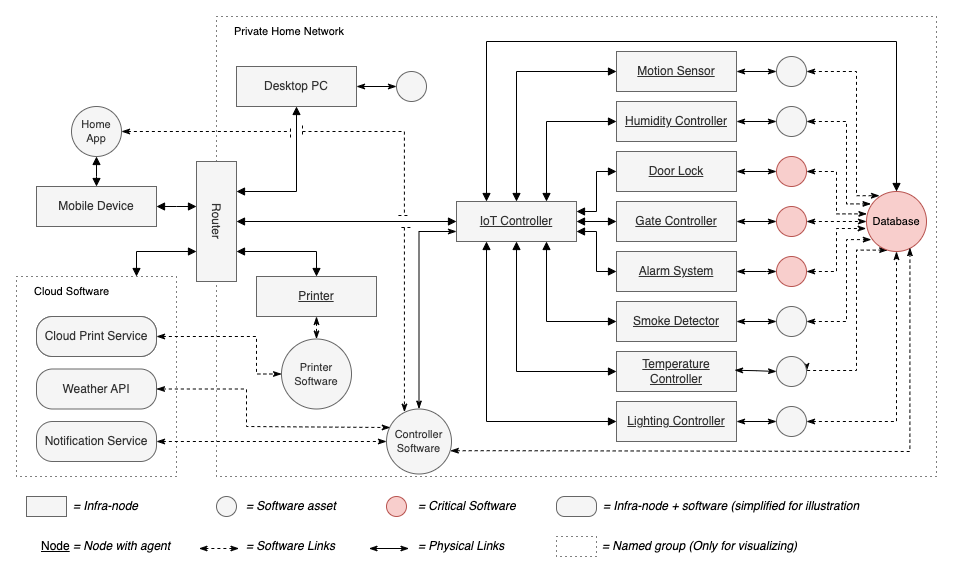
\includegraphics[width=0.9\textwidth]{_content/infrastructure}
    \caption{The infrastructure that is used in the experiments.}
    \label{fig:infrastructure}
\end{figure}

The infrastructure in figure \ref{fig:infrastructure} tries to mimic a smart-home environment, with a set of IoT devices such as the alarm system, door lock, and motion sensor. Each of these devices runs a specific software asset which is depicted by the smaller circles next to them. Next to the IoT devices, several 'common' devices are present, such as a printer, desktop, and router. The heart of the smart home is the IoT Controller, which is responsible for managing the other devices through the Controller Software. The Software assets marked with a red border are critical assets, which means that compromising these assets could have a significant impact. For example, a compromised door lock could allow an attacker to enter the house. The Cloud Software on the left of figure \ref{fig:infrastructure} is designed to have multiple entry points into the private network. This is done to mimic a real-world scenario where the cloud software is hosted on a cloud provider and is accessible through the internet. One example would be the usage of a cloud-based printer provider that allows users to print documents from outside of the network.


\subsection{Metrics and Evaluation}
\label{ssec:metrics}
During each of the experiments, several metrics are measured. These metrics are used to evaluate the results of the experiments and help answer the research question. 

The metrics we've defined can be categorized by effectiveness and efficiency. Effectiveness metrics measure how well the system can identify and mitigate risks. Efficiency metrics measure how well the system is able to do this with the least amount of resources. The metrics that are measured are shown in Table \ref{table:metrics-groups}.

\begin{table}[H]
    \centering
    \begin{tabular}{l|l}
        \textbf{Effectiveness}            & \textbf{Efficiency}            \\
        Total \# of risk identified       & Total \# of messages exchanged \\
        \# of remaining risks             & \# of adaptations              \\
        The sum of damages of remaining risk & Time spent auctioning  \\
                                          & Time spent adapting            \\
    \end{tabular}
    \caption{\label{table:metrics-groups}Overview of the metrics that are measured, grouped by either effectiveness or efficiency.}
\end{table}


The metrics are defined as follows:

\begin{description}
    \item[Sum of damages for remaining risks] The sum of the damage for the risks that have not been mitigated by the agents during the epoch. This can also be seen as the overall damage to the system. It is one of the key indicators of the system's performance. In essence, it is the metric that we are trying to minimize. The damage of a risk is calculated by multiplying the probability of the risk with the damage of the critical software component, as explained in Section \ref{ssec:adrian}. 
    % \comment{Zoltan}{I think this should be weighted by the probability of those risks}
    \item[Number of adaptations] The number of adaptations performed by the agents during the epoch.
    \item[Time spent auctioning] The time spent by the agents on auctioning. This time is measured from the moment an auction is initiated, or when an auction is joined, until the auction is finished. 
    \item[Time spent adapting] The time spent by the agents applying adaptations. This time is measured from the moment a proposal is accepted until the adaptation is finished.
    \item[Total number of messages exchanged] The total number of messages exchanged between agents during the epoch.
    \item[Total number of risks identified] The total number of risks identified by the agents during the epoch.
    \item[Number of remaining risks] The number of risks that have not been mitigated by the agents during the epoch.
\end{description}

\subsection{Controls and Variables}
\label{ssec:controls-variables}
% \begin{quote}\textcolor{red}{
%     Discuss any controls or variables that were taken into account to ensure the validity and reliability of your results. This could include experimental controls, randomization, and addressing potential confounding factors.
% }\end{quote}

When implementing the experiments, several controls and variables have been taken into account to ensure the validity and reliability of the results. The infrastructure, each scenario, and each feature set on its own can be seen as a bundle of variables, as they each heavily influence the characteristics of the experiments. 

% Talk about:
% - Fake timeouts/delays
% - Knowledge sharing depth/distance

\label{sssec:simulation-time}
One of the less trivial variables is the simulation time. During the simulation, we are (to some extent) in control over the time in the simulation that passes. This means that we can simulate a number of events that would take a long time in real life, in a matter of seconds. This is especially useful for  experiments where the infrastructure is growing over time. In real life, this would take a long time, but in the simulation, we can simulate this in a matter of seconds. This allows us to test the system in a more realistic scenario, without having to wait for a long time.

There is a limit to the speed-up that can be achieved in the simulation as the processing of certain events is not instantaneous. For example, doing the risk assessment of a node takes time. In a real-world scenario, this processing time (sub milliseconds) is negligible compared to the time messages take to travel over the network (100-1000 milliseconds) and the execution of adaptations (which take several hours to complete). However, in our simulation this processing time stays constant, and thus this processing time becomes more significant. To counter this, configurable delays were implemented to get a more realistic simulation. 
Places where these delays are implemented are for example the delivery of network-messages and the execution of adaptations. 

\label{sssec:knowledge-depth}
In the ADRIAN concept document by Mann and Smolka \cite{mann2023ADRIAN}, the concept of knowledge sharing depth/distance is mentioned.  This means that we can control how far agents can share their knowledge. This is done by setting a maximum distance between agents. This distance is defined as the number of hops a message can be sent between agents. This means that if the distance is set to 1, agents are only able to share knowledge with their direct neighbors. If the distance is set to 2, agents can share knowledge with their direct neighbors and the neighbors of their neighbors. During the experimentation, it is set to 1 and is not changed throughout the experiments, more on this in Section \ref{sec:future-research}.

\label{sssec:risk-rules}
As explained in Section \ref{ssec:adrian}, risk rules are used to identify risks and their probabilities in the infrastructure. These risk rules are what define attack graphs. In the experiments, we use the same set of risk rules for each experiment. This means that each experiment can identify the same risks.

Each agent allows for a handful of other variables, such as the strategies to select a risk for auctioning, or the best proposal in an auction. These strategies are not changed throughout the experiments but could be noteworthy for future research.

% \subsection{Baseline Experiment}
% % - No communication, no cooperation
% % - Predefined Infrastructure, same as other experiments
% % - Measure:
% %   - Number of adaptations
% %   - Total number of risks identified
% %   - Number of remaining risks
% %   - Sum of the damage for remaining risks

% % Mitigations take time, also communication. This should be discussed and used in the experiment.
% % Check costs of a mitigation

% \comment{Zoltan}{Arent these metrics collected in all experiments}The baseline experiment is conducted to measure metrics such as the number of adaptations and the number of risks identified. In this experiment Agents are not able to communicate with each other, and are not able to cooperate. 

% When the experiment has started, the agents are allowed to adapt their own properties and software components. However, the agents are not able to share knowledge and otherwise communicate with each other. To make the experiment easier to manage the \code{ExperimentManager} still is able to send messages to the agents, but the agents are not able to send messages to each other. \comment{Zoltan}{and also not able to cooperatively discover risks that require a global view I guess} Agents to being able to cooperate means that they are not able to join in auctions and therefore not able to work together to mitigate risks. A schematic overview of the experiment is shown in Figure \ref{fig:baseline}.

% \begin{figure}[H]
%     \centering
%     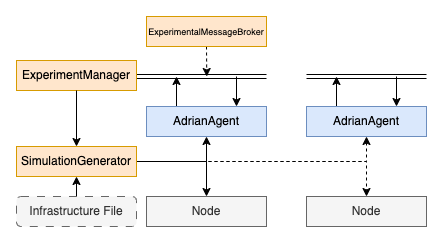
\includegraphics[width=0.8\textwidth]{_content/adrian-experiment-0}
%     \caption{Schematic overview of the baseline experiment, where multiple Agents are disconnected from one another.}
%     \label{fig:baseline}
% \end{figure}
% \comment{Zoltan}{It's not fully clear what this figure conveys. What do the individual symbols mean? In general, it is a good idea to explain all figures in the text, because they are often not as self-explanatory as you might think.}

% \subsection{Experiment 1: Risk Analysis}
% % - Communication, no cooperation
% % - Predefined Infrastructure, same as other experiments
% % - Measure:
% %   - Number of adaptations
% %   - Total number of messages exchanged
% %   - Total number of risks identified
% %   - Number of remaining risks
% %   - Sum of the damage for remaining risks

% The first experiment is conducted to measure the effect of communication between agents. In this experiment agents are able to communicate with each other, \comment{Zoltan}{I think you mean this only for mitigation, not for risk identification?} but are not able to cooperate. 

% When the experiment has started, the agents are allowed to adapt their own properties and software components. The agents are also able to share knowledge at a distance of \( D_{knowledge} \). In this experiment Agents are still not able to cooperate on mitigating risks, which is achieved by not allowing Agents to initiate or join auctions. A simplified overview of the experiment is shown in Figure \ref{fig:experiment-1}.

% \begin{figure}[H]
%     \centering
%     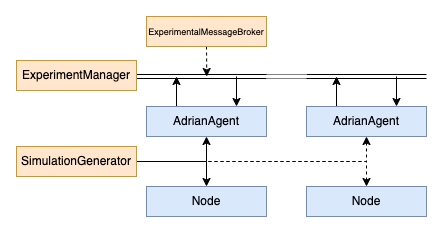
\includegraphics[width=0.8\textwidth]{_content/adrian-experiment-1}
%     \caption{Schematic overview of the first and second experiment, depicting the way multiple Agents are connected to each other and are controlled by the \code{ExperimentManager}.}
%     \label{fig:experiment-1}
% \end{figure}
% \comment{Zoltan}{It's not easy to spot the difference between this and the previous figure, like in a puzzle. Please make the life of your readers easier.}

% This experiment is repeated multiple times, with different values for \( D_{knowledge} \). The values for \( D_{knowledge} \) are 1, 2, and 3. The results of this experiment are compared to the results of the baseline experiment.

% \subsection{Experiment 2: Risk Mitigation}
% % - Communication, cooperation
% % - Predefined Infrastructure, same as other experiments
% % - Measure:
% %   - Number of adaptations
% %   - Total number of messages exchanged
% %   - Total number of risks identified
% %   - Number of remaining risks
% %   - Sum of the damage for remaining risks

% The second experiment is conducted to measure the effect of cooperation between agents. In this experiment agents are able to communicate with each other, and are able to cooperate. 

% When the experiment has started, the agents are allowed to adapt their own properties and software components. The agents are also able to share knowledge at a distance of \( D_{knowledge} \). Additionally, in this experiment Agents are able to cooperate on mitigating risks, which is achieved by allowing Agents to initiate and join auctions. The overview of this experiment is shown in Figure \ref{fig:experiment-1}.

% As with the first experiment, this experiment is repeated multiple times, with different values for \( D_{knowledge} \). The values for \( D_{knowledge} \) are 1, 2, and 3. The results of this experiment are compared to the results of the baseline experiment and the first experiment.
